%%%%%% DON'T MODIFY STARTING HERE
\newpage
\section*{5. Cameras \& Mirobot}

In addition to the Mirobot, you will also work with the RealSense D400 series of sensors.
These sensors have an RGB camera as well as a 3D depth sensor.
In this exercise you will learn how to interface with these cameras and calibrate them relative to the robot.

\paragraph{5A.} Install OpenCV and RealSense API as instructed below. Attach a final screenshot of your prompt after step 3.
\begin{enumerate}
    \item Activate your conda environment: \texttt{conda activate 52-O}
    \item Install OpenCV: \texttt{conda install -c conda-forge opencv}
    \item Install the \href{https://github.com/IntelRealSense/librealsense/tree/master/wrappers/python#installation}{\texttt{pyrealsense2}} library: \texttt{pip install pyrealsense2}
\end{enumerate}

\paragraph{5B.} Connect the camera to your machine.\\

The camera uses a USB 3 connection and a USB-C connector. Please connect \textbf{both} the camera and the robot into your machine.
Please use the provided USB hub, if needed.
Attach a photo of the camera and robot attached to your machine.

\paragraph{5C.} Visualize camera output using OpenCV.

\begin{enumerate}
    \item Run the Python script \texttt{code/q5c\_1.py}. Attach a screenshot of what you see when you run this code.
    \item Run the Python script \texttt{code/q5c\_2.py}. Attach a screenshot of what you see when you run this code.
\end{enumerate}

\paragraph{5D.} Camera calibration.
Follow this \href{https://docs.opencv.org/3.4/dc/dbb/tutorial_py_calibration.html}{tutorial} to understand camera intrinsics and extrinsics calibration.
Use the \texttt{calibrateCamera} function in OpenCV and implement calibration of both intrinsics and extrinsics.
Please attach your code and the intrinsics matrix (\texttt{cameraMatrix}) for the RGB camera in Intel RealSense.

You may want to combine code from 5C for this part.
A printed 9x6 checkerboard pattern is available in your workspace.
You can also find it \href{https://drive.google.com/file/d/1Hk-U4xiAmZnrf3qGziQWBW7YbEMFTWgY/view?usp=sharing}{here}.
%%%%%% DON'T MODIFY UNTIL HERE
 
\newpage
\paragraph{Answers.}
Please do not exceed the height provided for each answer image.
%%%%%% YOU ANSWER STARTS HERE

% NOTE: MAKE SURE YOU DON'T CHANGE THE HEIGHT OF IMAGES
% NOTE: MAKE SURE TO REMOVE THE 'draft' OPTION FOR includegraphics BELOW. OTHERWISE, YOU WILL NOT SEE YOUR IMAGES.

\paragraph{5A. Install OpenCV and RealSense API.}
\begin{center}
    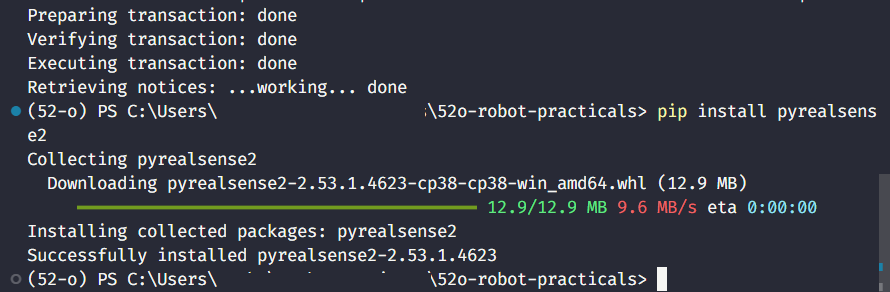
\includegraphics[height=2in]{image/5a_vision.png}
\end{center}

\paragraph{5B. Connect Camera to your machine.}
\begin{center}
    \includegraphics[draft,height=2.5in]{YOUR\_ANSWER.png}
\end{center}

\newpage
\paragraph{5C. Visualize using OpenCV.}
\begin{center}
    \includegraphics[draft,height=2.5in]{YOUR\_ANSWER.png}
\end{center}

\paragraph{5D. Camera Calibration.}
%
\begin{minted}{python}
    var = 'YOU CODE GOES HERE'
\end{minted}

Please also report the matrix stored in the \texttt{cameraMatrix} return variable of the \texttt{calibrateCamera} function.


\newpage
\paragraph{Additional Space.}
Please do not exceed this page for this question.
%%%%%% YOU ANSWER ENDS HERE
